% Preamble
\documentclass[12pt]{article}

% Packages
\usepackage[left=3.0cm, right=1.5cm, top=2.0cm, bottom=2.0cm]{geometry}

\usepackage[utf8]{inputenc}
\usepackage[T2A]{fontenc}
\usepackage[russian]{babel}
\usepackage{amsmath, amsfonts, amssymb}
\usepackage{graphicx}
\usepackage{wrapfig}
\usepackage{fancyhdr}
\usepackage[shortlabels]{enumitem}
\usepackage{svg}
\usepackage{amstex}
\usepackage{colortbl}
\usepackage{bm}

\renewcommand{\vec}{\textbf}
\newcommand{\cross}{\times}

\pagestyle{fancy}
\fancyhead[L]{Работа №4.1.1}
\fancyhead[R]{Белинский Т.Д.\quad Б05-206}

% Document
\begin{document}
    \section*{4.1.1. Изучение центрированных оптических систем}
    \ \par
    \textbf{Цель работы:} изучить методы определения фокусных расстояний
    линз и сложных оптических систем; определить характеристики оптической системы, составленной из тонких линз; изучить недостатки
    реальных линз -- сферическую и хроматическую аберрации.


    \textbf{Оборудование:} оптическая скамья с набором рейтеров, положительные и отрицательные линзы, экран, осветитель с ирисовой
    диафрагмой, зрительная труба, светофильтры, кольцевые диафрагмы, линейка.


    \subsection*{Теоретическая часть}
    \ \par
    \textbf{Измерение фокусного расстояния по методу Аббе} основано на определении поперечного увеличения для нескольких (не менее двух) различных положений предмета,
    находящегося на оптической оси исследуемой оптической системы.
    На рис. 1 представлена соответствующая схема эксперимента.
    \begin{figure}[h]
        \centering
        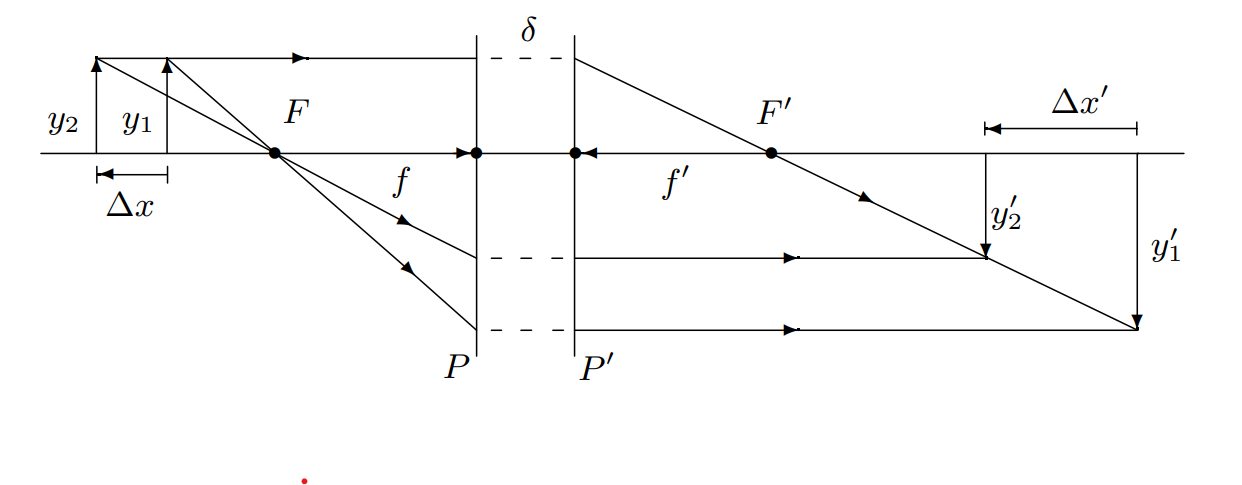
\includegraphics[width=0.6\linewidth]{pic/1}
        \caption{}
        \label{fig:1}
    \end{figure}
    фокусное расстояние системы можно выразить через положения предмета и соответствующие увеличения следующим образом:
    \[f = \frac{\Delta x}{\Delta (y/y')} = -\frac{\Delta x'}{\Delta(y'/y)}.\]
    Здесь $\Delta x = x_2 - x_1$ -- смещение предмета, $\Delta x' = x'_2 - x'_1$ --
    соответствующее ему перемещение изображения, $\Delta (y'/y) = y_2/y'_2 - y_1/y'_1$ --
    приращение поперечного увеличения, а $\Delta (y/y')$ — приращение величины,
    обратной поперечному увеличению.
    Для повышения точности измерений следует выбирать такие смещения $\Delta x$, чтобы увеличения заметно
    отличались друг от друга.
    С целью уменьшения случайной ошибки, возникающей при фокусировке изображения,
    измерения следует проводить несколько раз, усредняя полученные данные.

    \textbf{Определение фокусного расстояния собирающих линз и сложных
    оптических систем по методу Бесселя.}
    Схема метода Бесселя для случая, когда $n = n'$ и $f' = -f$, представлена на рис. 2.
    Она основана на том, что при заданном расстоянии
    $L$ между предметом и экраном представляет собой
    квадратное уравнение относительно расстояния $s$ от главной плоскости пространства предметов до предмета $(s < 0)$:
    \[-\frac{1}{s}+\frac{1}{L-\delta+s} = \frac{1}{f},\]
    имеющее при условии $L > 4f +\delta$ решения $s_1$ и $s_2$, показанные на рис. 2,
    где $\delta$ -- расстояние между главными плоскостями системы (линзы).
    \begin{figure}[h]
        \centering
        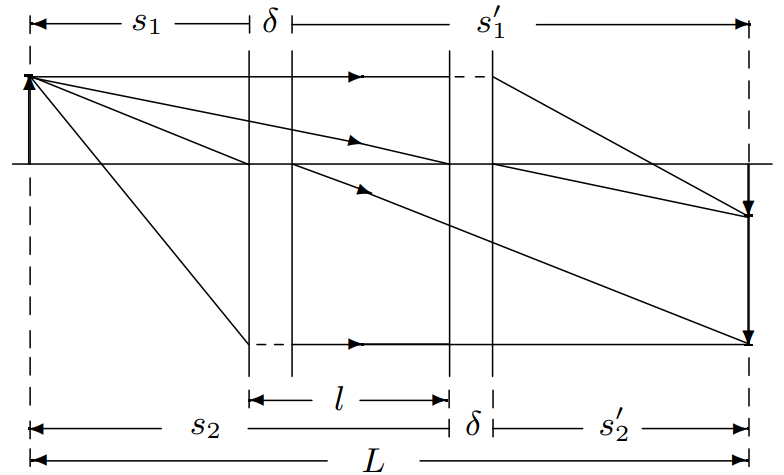
\includegraphics[width=0.6\linewidth]{pic/2}
        \caption{}
        \label{fig:2}
    \end{figure}

    С учётом симметрии и направлений измерения расстояний,
    положения предметов определяются соотношениями $s'_2 = -s_1$ и $s'_1 = -s_2$.
    Для расстояния $L$ между предметом и экраном и расстояния $l$ между двумя положениями системы (линзы)
    получаем: $L - \delta = s'1 - s1$, $l = -s_2 + s_1 = s_1 + s'_1$.
    Отсюда следует, что
    \[s_1 = -\frac{1}{2}(L-\delta-l),\quad s'_1=\frac{1}{2}(L - \delta + l).\]
    После несложных преобразований находим выражение
    \[f = \frac{(L-\delta)^2 - l^2}{4(L  - \delta)}\]


    \subsection*{Результаты и обработка}
    \begin{enumerate}
        \item Измеряем фокусы линз, полученные данные приведены в таблице 1.
        Для рассеивающей линзы 4.5 $l = 197$ мм $a_0=290$  мм
        \[f = l - a_0 = (-93\pm 2)\ \text{мм}.\]

        \item Для линзы 4.2 измерим фокусное расстояние методом Бесселя ($L = 600$ мм), полученные данные собраны в таблице 2.
        Оценка по формуле тонкой линзы:
        \[f_{\text{тл}} = \frac{1}{\frac{1}{s_1} + \frac{1}{L - s_1}} = (126.3 \pm 0.2)\ \text{мм};\]
        оценка методом Бесселя:
        \[f_{\text{мб}} = \frac{L^2 - l^2}{4L} = (124.8 \pm 0.6)\ \text{мм}.\]

        \item Для той же линзы 4.2 измерим фокусное расстояние методом Аббе, полученные данные собраны в таблице 3.
        \[f_1 = \frac{\Delta x'}{\frac{y_1}{y_0} - \frac{y_2}{y_0}} = (123 \pm 2)\ \text{мм};
        \quad f_2 = \frac{\Delta x}{\frac{y_0}{y_2} - \frac{y_0}{y_1}} = (127 \pm 3)\ \text{мм}\]
        Тогда:
        \[f = \frac{f_1 + f_2}{2} = (125 \pm 2)\ \text{мм}\]

        \item Определим увеличение телескопа Галилея, собранного из исследуемых линз (линзы 4.5, 4.3)
        \[\gamma_{\text{эксп}} = \frac{a}{a_0} = \frac{100/300}{57/310} = (1.8\pm0.1)\]
        \[\gamma_{\text{теор}} = \frac{f_{\text{об}}}{f_{\text{ок}}} = \frac{180}{93} = (1.9\pm0.1)\]
        \[D_{\text{об}} = (14.0\pm0.5)\ \text{мм},\ D_{\text{ок}} = (7.0\pm0.5)\ \text{мм}
        \quad \gamma = \frac{D_{\text{об}}}{D_{\text{ок}}} = (2.0 \pm0.1)\]

        \item Оценим увеличение микроскопа, собранного из исследуемых линз (линзы 4.1, 4.2, $L = (38.00\pm0.05)$ см,
        $a = (40.0\pm0.5)$ мм, $a_0 = (17\pm0.5)$ мм)
        \[\gamma_{\text{эксп}} = \frac{a}{a_0} \frac{L}{f_{\text{кол}}} = (2.3\pm0.1)\]
        \[\gamma_{\text{пр}} = \frac{L - f_{\text{ок}}}{f_{\text{ок}}}\frac{\Delta}{f_{\text{об}}} = (2\pm0.1)\]
    \end{enumerate}
    \begin{table}[b]
        \centering
        \caption{Фокусы собирающих линз}
        \label{tab:1}
        \begin{tabular}{|lcccc|}
            \hline
            №   & $f_1$ мм & $f_2$ мм & $f$ мм & $\Delta$ мм \\\hline
            4.1 & 80       & 83       & 81.5   & 2           \\
            4.2 & 130      & 132      & 131.0  & 1           \\
            4.3 & 183      & 179      & 181.0  & 2           \\
            4.4 & 257      & 252      & 254.5  & 3           \\\hline
        \end{tabular}
    \end{table}

    \begin{table}[b]
        \centering
        \caption{Метод Бесселя}
        \label{tab:2}
        \begin{tabular}{|ccc|}
            \hline
            $s_1$ мм & $s_2$ мм & $l$ мм \\\hline
            181      & 430      & 249    \\
            180      & 423      & 243    \\\hline
        \end{tabular}
    \end{table}

    \begin{table}[b]
        \centering
        \caption{Метод Аббе}
        \label{tab:3}
        \begin{tabular}{|ccccc|}
            \hline
            $y_0$ мм & $y_1$ мм & $y_2$ мм & $\Delta x$ & $\Delta x'$ \\\hline
            20       & 72       & 46       & 20         & 160         \\\hline
        \end{tabular}
    \end{table}
\end{document}